\documentclass[11pt,a4paper,oneside]{book}
\usepackage{lecturestyle}


\begin{document}


\title{MATH6103 Differential \& Integral Calculus \\
Notes in Brief \\[1in]
Department of Mathematics, \\
University College London \\[1.5in]}
\author{\Large Matthew Scroggs \\
web: \texttt{www.mscroggs.co.uk/6103} \\
e-mail: \texttt{matthew.scroggs.14@ucl.ac.uk}}
\date{\Large Spring 2016}

\frontmatter
\maketitle
\tableofcontents

\mainmatter

\chapter*{Using These Notes}
These notes are intended as a revision aid. I started with the full lecture notes of the course and taken out all
unnecessary detail, examples, etc.\ to leave a minimal outline of the course. If you need more detail on a topic,
look at the relevant section in the full notes!

Throughout these notes in brief, you will find boxes that look like this:

\begin{gce}
A-level C1 Differentiation
\end{gce}

These boxes contain references to the parts of GCSE and A-level maths that are relevant to the section. These may
be useful as there is a great range of GCSE and A-level revision material online. These are all based on the syllabus 
of the EdExcel exam board, as this is the one I am familiar with. Other exam boards are mostly the same.

\chapter{Functions}
\begin{gce}
A-level C1 functions
\end{gce}
$\mathbb{Z}=\{\text{all whole numbers}\}=\{\dots,-2,-1,0,1,2,\dots\}$\\
$\mathbb{N}=\{\text{all positive whole numbers}\}=\{0,1,2,3,\dots\}$\\
$\mathbb{R}=\{\text{all real numbers}\}$

\hrule

$f:A\rightarrow B$\\
$A$ is the \textbf{domain} of $f$. $B$\footnote{or a subset of $B$} is the \textbf{range} of $f$.

If \(x\not=y\) implies \(f(x)\not=f(y)\), the function is \textbf{one-to-one}.\\
Otherwise, the function is \textbf{many-to-one}.

If $f(-x)=f(x)$, $f$ is \textbf{even}.\\
If $f(-x)=-f(x)$, $f$ is \textbf{odd}.

If $f(x+T)=f(x)$ for all $x$, then $f(x)$ is a \textbf{periodic function} with period $T$.

\textbf{Vertical/horizontal asymptotes} are vertical/horizontal lines that the function approached but never reaches.

\section{Polynomials}

A polynomial is a function $P$ with a general form
$$P(x)=a_0 + a_1x + a_2x^2+\dots+a_nx^n$$

\subsection{Some polynomial degrees}
\subsubsection{Degree 0} This polynomial is simply a constant.

\subsubsection{Degree 1} $P_1(x)= ax+b$ ($a\ne 0$). $a$ is the gradient. $b$ is the $y$-intercept

\subsubsection{Degree 2} $P_2(x)=ax^2 +bx +c$, $a\ne 0$ are called quadratics.
\begin{gce}
GCSE quadratics\\
A-level C1 quadratics
\end{gce}

%%%%%%%%%%%%%%%%%%%%%%%%%%%%%%%%%%%%%%%
\textbf{1. Factorising}

\begin{example}
\begin{align*}
P(x)&=x^2-3x +2
&=(x-2)(x-1)
\end{align*}
The solutions of $P(x)=0$ are $x=2$ and $x=1$.
\end{example}

%%%%%%%%%%%%%%%%%%%%%%%%%%%%%%%%%%%%%%%
\textbf{2. Completing the square}

\begin{example}
\begin{align*}
P(x)&=x^2-3x+2\\
&=\left(x-\tfrac{3}{2}\right)^2-\left(\tfrac{-3}{2}\right)^2+2
\end{align*}
\begin{align*}
\left(x-\tfrac{3}{2}\right)^2-\left(\tfrac{-3}{2}\right)^2+2&=0\\
\left(x-\tfrac{3}{2}\right)^2&=\tfrac{1}{4}\\
x-\tfrac{3}{2}&=\pm \tfrac{1}{2}\\
x&=1\text{ or }2
\end{align*}
\end{example}

\textbf{3. The quadratic formula}

\begin{equation*}
x=\frac{-b \pm \sqrt{b^2-4ac}}{2a}.
\end{equation*}

\subsubsection{Degree $\ge 3$}
\begin{gce}
A-level C2 Remainder theorem
\end{gce}
\begin{theorem}[Factor theorem]
$$P(a) = 0\quad \text{if and only if}\quad P(x)=(x-a)Q(x)$$
\end{theorem}

\section{Exponentials}
\begin{gce}
GCSE Indices and powers
\end{gce}
\begin{in_a_box}
\begin{align*}
a^{x+y}&=a^x\cdot a^y\\
\left( a^x \right)^y&=a^{xy}\\
a^x \cdot b^x &= \left( ab \right)^x\\
a^0&=1\\
a^{-x}&=\frac{1}{a^x}\\
a^\frac{1}{n} &= \sqrt[n]{a}\\
a^\frac{m}{n} &= \left(\sqrt[n]{a}\right)^m
\end{align*}
\end{in_a_box}

\section{Trigonometric functions}
\subsection{Measuring angles}
\begin{gce}
GCSE Trigonometry\\
A-level C3 Radians
\end{gce}
\begin{in_a_box}
$$\begin{array}{rcccl}
1\text{ turn}&=&360^{\circ}&=&2\pi\,\mbox{rad}\\
\frac{1}{2}\text{ turn}&=&180^{\circ}&=&\pi\,\mbox{rad}
\end{array}$$
\end{in_a_box}
``SOH CAH TOA"

\subsection{Properties of sin, cos and tan}
\begin{gce}
A-level C2 Trigonometry\\
A-level C3 Trigonometry
\end{gce}
$\cos^2\theta+\sin^2\theta=1$

$\cos$ and $\sin$ are periodic functions with period $2\pi$ (i.e. for any $x$, $\cos(x+2\pi)=\cos x$, $\sin(x+2\pi)=\sin x$).

$\cos : \mathbb{R}\to[-1,1]$ and $\sin : \mathbb{R}\to[-1,1]$.

$\cos$ is an even function. $\sin$ is an odd function.

$\cos$ and $\sin$ are the same shape but shifted by $\pi/2$, which means
$$\cos\left(\theta-\frac{\pi}{2}\right)=\sin\theta$$
$$\sin\left(\theta+\frac{\pi}{2}\right)=\cos\theta$$

$$\cos(\theta+\phi)=\cos\theta\cos\phi-\sin\theta\sin\phi$$
$$\sin(\theta+\phi)=\sin\theta\cos\phi+\cos\theta\sin\phi$$

$$\sin2\theta = 2\sin\theta\cos\theta$$
$$\cos2\theta = 1-2\sin^2\theta$$
$$\cos2\theta = 2\cos^2\theta-1$$

$$\cos^2\left(\frac{\alpha}{2}\right)=\frac{1+\cos\alpha}{2}$$
$$\sin^2\left(\frac{\alpha}{2}\right)=\frac{1-\cos\alpha}{2}$$

$\tan$ has vertical asymptotes at $\theta=\frac{\pi}{2}\left(2N-1\right)$ for $N\in\mathbb{Z}$.

$\tan : \mathbb{R}\setminus\{\frac{\pi}{2}(2N-1):N\in\mathbb{Z}\}\to\mathbb{R}$

$\tan$ is periodic with period $\pi$.

$$\tan(\theta+\phi)=\,\, \frac{\tan\theta+\tan\phi}{1-\tan\theta \tan\phi}$$

The secant, cosecant and cotangent functions are defined as 
\[\sec x=\frac{1}{\cos x},\quad \mathrm{cosec} x=\frac{1}{\sin x},\quad \mathrm{cot} x=\frac{1}{\tan x}. \]

$$1+\tan^2 x = \sec^2 x.$$

\begin{center}
\begin{tabular}{|c|c||c|c|c|}
\hline
\textbf{Angle (\degs)} & \textbf{Angle (\rads)} & \textbf{sin} & \textbf{cos} & \textbf{tan}\\\hline
0&0&0&1&0\\\hline
30&$\frac{\pi}{6}$&$\frac{1}{2}$&$\frac{\sqrt{3}}{2}$&$\frac{3}{\sqrt{3}}$\\\hline
45&$\frac{\pi}{4}$&$\frac{1}{\sqrt{2}}$&$\frac{1}{\sqrt{2}}$&1\\\hline
60&$\frac{\pi}{3}$&$\frac{\sqrt{3}}{2}$&$\frac{1}{2}$&$\sqrt{3}$\\\hline
90&$\frac{\pi}{2}$&1&0&$\infty$\\\hline
\end{tabular}
\end{center}

\section{Polar co-ordinates}
\begin{figure}[H]
    \includegraphics[scale=0.5]{img/polar_def.jpg}
    \centering
  \caption{Polar co-ordinates are given by $r$ and $\theta$.}
\end{figure}

\begin{in_a_box}
$$x=r\cos\theta$$
$$y=r\sin\theta$$
\end{in_a_box}

\chapter{Differentiation}
$$\text{gradient}=\frac{\text{change in }y}{\text{change in }x}$$

\section{Finding the gradient}
\begin{gce}
A-level C1 Differentiation\\
A-level C2 Differentiation\\
A-level C3 Differentiation
\end{gce}
\begin{definition}
Differentiation by first principles:
$$f'(c)=\lim_{h\rightarrow 0}\frac{f(c+h)-f(c)}{h}.$$
\end{definition}

\section{Some common derivatives}

\textbf{IMPORTANT: Always use radians!}

\begin{tabular}{|c | c|}
\hline
$f(x)$&$f'(x)$\\\hline
$x^n$&$nx^{n-1}$\\
$\sin x$&$\cos x$\\
$\cos x$&$-\sin x$\\
$\tan x$&$\sec^2 x$\\
\hline
\end{tabular}
\section{Rules for differentiation}
\begin{gce}
A-level C4 Differentiation
\end{gce}
\begin{thing}{The sum rule}
\[\frac{d}{dx}\left( f(x)+g(x)\right)=\frac{d}{dx}\left(f(x)\right)+\frac{d}{dx}\left(g(x)\right)\]
\end{thing}

\begin{thing}{The product rule}
\[\frac{d}{dx}\left( f(x)g(x) \right) = \frac{d}{dx}\left(f(x)\right)g(x) + f(x)\frac{d}{dx}\left(g(x)\right)\]
\end{thing}

\begin{thing}{The chain rule}
\[\frac{d}{dx}\left( f(g(x) ) \right) = f'(g(x))g'(x)\]
\end{thing}

\begin{thing}{The quotient rule}
\[\frac{d}{dx}\left( \frac{f(x)}{g(x)} \right) = \frac{f'(x)g(x) - f(x)g'(x)}{(g(x))^2}\]
\end{thing}

\section{Polar co-ordinates}
The chain rule can be rearranged to give:

\begin{in_a_box}
\[\frac{dy}{dx}=\frac{dy/dt}{dx/dt}\]
\end{in_a_box}

\begin{example}
$x=t^2 + 4$; $y=e^t$
\begin{align*}
\frac{dy}{dx}&=\frac{dy/dt}{dx/dt}\\
&=\frac{e^t}{2t}\\
\end{align*}
\end{example}

\section{Uses of differentiation}
\subsection{Finding the gradient at a point}
The gradient of $f$ at $x=k$ is $f(k)$.

\subsection{Finding the maximum and minimum points}
\begin{itemize}
\item Local maximum $$f'(x)=0$$ $$f''(x)<0$$
\item Local minimum $$f'(x)=0$$ $$f''(x)>0$$
\item Need more information $$f'(x)=0$$ $$f''(x)=0$$
\end{itemize}

\section{Differentiating inverse functions}

\begin{definition}
$f^{-1}$ is the inverse of $f$: $$f^{-1}(f(x))=x$$
\end{definition}

\note{Sometimes, $\arcsin$, $\arccos$ and $\arctan$ are used to represent $\sin^{-1}$, $\cos^{-1}$ and $\tan^{-1}$.}

\begin{thing}{Finding the derivative of an inverse}
$$\frac{d}{dx}\left(f^{-1}(x)\right)=\frac{1}{f'(f^{-1}(x))}$$
\end{thing}

\begin{in_a_box}
$$\frac{dy}{dx}=\frac{1}{\frac{dx}{dy}}$$
\end{in_a_box}

\chapter{Exponentials and Logarithms}
\section{Exponentials}
\begin{gce}
A-level C3 Exponentials and Logarithms
\end{gce}
 \[f(x)=a^{x},\]
 
\begin{figure}[H]
    \hspace{0.2cm}
    \subfigure[$y=2^x$]{\label{fig:eponential-2-power-x}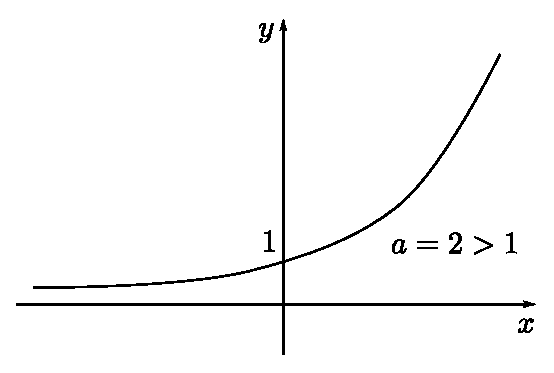
\includegraphics[scale=0.6]{img/eponential-2-power-x}}
    \hspace{2.0cm}
    \subfigure[$y=\left(\frac{1}{2}\right)^x$]{\label{fig:eponential-half-power-x}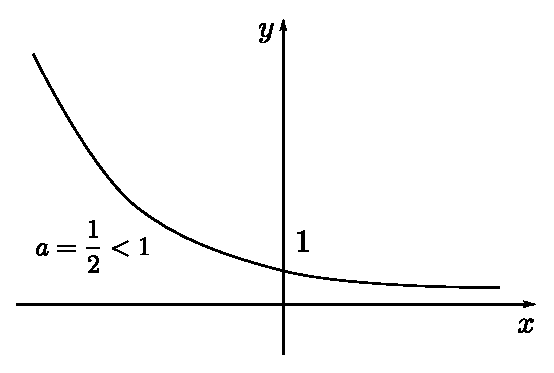
\includegraphics[scale=0.6]{img/eponential-half-power-x}} \\
    \centering
\end{figure}

$e\approx2.718281828459\dots$

\begin{definition}
$f(x)=e^x=\exp(x)$ is the \textbf{exponential function}.
\end{definition}

\begin{thing}{Property}
\[\frac{d}{dx}(e^x)=e^x.\]
\end{thing}

\section{Logarithms}
\begin{gce}
A-level C2 Exponentials and Logarithms\\
A-level C3 Exponentials and Logarithms
\end{gce}
\begin{definition}
The inverse of $a^x$ is $\log_a x$.
\end{definition}

\begin{thing}{Laws of Logs}
\begin{itemize}
\item[1.] $\log_a(MN)=\log_aM + \log_aN$.
\item[2.] $\log_a(M^p)=p\log_aM$.
\end{itemize}
\end{thing}

\begin{example}
Find $x$, given $3^x=7$.
\begin{align*}
\ln(3^x)&=\ln7\\
x\ln 3&=\ln 7.\\
x&=\frac{\ln 3}{\ln 7}\\&\approx1.77
\end{align*}
\end{example}


\subsection{The natural logarithm}
\begin{gce}
A-level C3 Exponentials and Logarithms
\end{gce}
\begin{definition}
The inverse of $f(x)=e^x$ is the \textbf{natural logarithm}, $\ln x$.
\end{definition}

\begin{thing}{Property}
\[\frac{d}{dx}(\ln x)=\frac{1}{x}.\]
\end{thing}

\subsection{Differentiation of other logarithms}
\begin{gce}
A-level C3 Exponentials and Logarithms
\end{gce}
\begin{thing}{Property: Change of base}
\[\log_ax=\frac{\log_bx}{\log_ba}\]
\end{thing}
\begin{thing}{Property}
\[\frac{d}{dx}\left( \log_ax\right)=\frac{1}{x\ln a}.\]
\end{thing}

\section{Differentiation of other exponentials}
\begin{gce}
A-level C3 Exponentials and Logarithms
\end{gce}
\begin{in_a_box}
In general, for any positive constant $a$
\[\frac{d}{dx}(a^x)=a^x\ln a.\]
\end{in_a_box}

\chapter{Integration}
Integration = Finding the area under the curve.

\begin{theorem}[Fundamental Theorem of Calculus]
\[\int_a^b g'(x) \dx = g(a)-g(b)\]
\end{theorem}

\section{Finding integrals}
\begin{gce}
A-level C1 integration\\
A-level C2 integration\\
A-level C4 integration
\end{gce}
\begin{tabular}{|c|c|}
\hline
$f(x)$&$\int f(x)\dx$\\\hline
$ax^b$&$\frac{ax^{b+1}}{b+1}+c$\\
$\frac{1}{x}$&$\ln |x|+c$\\
$e^x$&$e^x+c$\\
$a^x$&$\frac{a^x}{\ln a}+c$\\
$\cos x$&$\sin x + c$\\
$\sin x$&$-\cos x + c$\\
\hline
\end{tabular}

\section{Rules for integration}
\begin{thing}{Sum Rule}
\begin{equation}
\int \left( f(x)+g(x) \right)\dx=\int f(x)\dx+ \int g(x)\dx
\end{equation}
\end{thing}
\begin{thing}{Multiplication by a constant}
\begin{equation}
\int K f(x)\dx=K\int f(x)\dx
\end{equation}
\end{thing}

\begin{thing}{A special case}
\[\int \frac{f'(x)}{f(x)}\dx=\ln(f(x))+c\]
\end{thing}


\begin{example}[Integration by Substitution]
\begin{gce}
A-level C4 Integration
\end{gce}
$$\int(2x+3)^{100}\dx$$
\[u=2x+3.\]
\[\frac{du}{dx}=2\]
\[dx=\frac{1}{2}\dx[u].\]
\begin{eqnarray*}
\int (2x+3)^{100}\dx &=& \int u^{100}\cdot \frac{1}{2}\dx[u] \\
&=& \frac{1}{2}\int u^{100}\dx[u] \\
&=& \frac{1}{2}\cdot\frac{1}{101}u^{101} \\
&=& \frac{1}{202}(2x+3)^{101}+c.
\end{eqnarray*}
\end{example}

\begin{thing}{Integration by Parts}
\begin{gce}
A-level C4 Integration
\end{gce}
\begin{equation*}
\int u\frac{dv}{dx}\dx=uv-\int v\frac{du}{dx}\dx.
\end{equation*}
\end{thing}

\subsection{Partial fractions}
\begin{gce}
A-level C4 Integration
\end{gce}
\begin{example}
\[\frac{1}{x^2-1}\]
\[x^2-1 = (x+1)(x-1)\]
\[\frac{1}{x^2-1}=\frac{A}{x-1}+\frac{B}{x+1},\]
\[1=A(x+1)+B(x-1)\]
Substituting in \(x=1\) gives \(1=2A.\)

Substituting in \(x=-1\) gives \(1=-2B.\)

$A=\tfrac12$; $B=-\tfrac12$.
\[\frac{1}{x^2-1}=\frac{1}{2(x-1)}-\frac{1}{2(x+1)}\]
\end{example}

\subsection{Trapezium method}
\begin{gce}
A-level C2 Integration\\
A-level C4 Integration
\end{gce}
This is a method for approximating an integral.

\begin{in_a_box}
$$\int_a^b f(x) \dx \approx \frac{h}2\left(f(a)+2f(a+h)+...+2f(a+(n-1)h)+f(b)\right)$$
\end{in_a_box}

\chapter{Differential Equations}

\section{First order differential equations}
\begin{gce}
A-level C4 Integration
\end{gce}
Here we will consider different techniques to solve first order ODEs.

\begin{definition}
A function $f(x,y)$ is \textbf{separable} if it can be written as
\[f(x,y)=g(x)h(y).\]
\end{definition}

\begin{example}[Separating the variables]
\[\frac{dy}{dx}=xy,\]
\[\frac{1}{y}\dx[y]=x\dx\]
$$\int\frac{1}{y}\dx[y]=\int x\dx$$
$$\ln y=\frac{1}{2}x^2 +C$$
\[y=e^{\frac{1}{2}x^2+C}=Ae^{\frac{1}{2}x^2},\quad A=e^C.\]
\end{example}

If boundary conditions are given, substitute them in to find the constant(s).

\subsection{Integrating factors}
\begin{gce}
A-level FP2 First Order Differential Equations
\end{gce}
\begin{definition}
The \textbf{integrating factor} of the ODE 
\[\frac{dy}{dx}+g(x)y=f(x).\]
is 
\[\exp\left({\int g(x)\dx}\right).\]
\end{definition}

\begin{example}
\[\frac{dy}{dx}+\frac{y}{x}=x.\]

The integrating factor is:
\begin{align*}
\exp\left(\int\frac{1}{x}\dx\right)
&=\exp\left(\ln x\right)\\
&=x
\end{align*}

Multiplying through by the integrating factor gives:
\[x\frac{dy}{dx}+y=x^2\]

Notice that: \[\frac{d}{dx}\left(xy\right) = x\frac{dy}{dx}+y\]

Therefore:
\begin{align*}
\frac{d}{dx}\left(xy\right) &= x^2\\
xy &= \int x^2\dx\\
&= \frac{x^3}{3} +c\\
y &= \frac{x^2}{3} +\frac{c}{x}\\
\end{align*}

\end{example}

\section{Complementary functions and particular integrals}
\begin{gce}
A-level FP2 Second Order Differential Equations
\end{gce}
\begin{definition}
When \(y=f(x) + cg(x)\) is the solution of an ODE, \(f\) is called the \textbf{particular integral} (P.I.) and \(g\) is called the \textbf{complementary function} (C.F.).
\end{definition}

\begin{enumerate}
\item The complementary function ($g$) is the solution of the homogenous ODE.
\item The particular integral ($f$) is any solution of the non-homogenous ODE.
\end{enumerate}

\subsection{Finding complementary functions}

Aim: find two independent solutions to 
\[\frac{d^2y}{dx^2} + A\frac{dy}{dx} + By = 0\]

\begin{definition}
\[\lambda^2+A\lambda+B=0\] is the \textbf{characteristic equation} or \textbf{auxiliary equation} of 
\[\frac{d^2y}{dx^2} + A\frac{dy}{dx} + By = 0.\]
\end{definition}

\subsubsection{Case 1: Two distinct real roots}
\[\lambda_1=\frac{-r+\sqrt{A^2-4B}}{2}\quad\text{ and }\quad \lambda_2=\frac{-r-\sqrt{A^2-4B}}{2}\]
\[g(x)=c_1e^{\lambda_1x}+c_2e^{\lambda_2x}.\]

\subsubsection{Case 2: Repeated root}
\[\lambda_1=\frac{A}{B}.\]
\[g(x)=(c_1+c_2x)e^{\lambda_1x}.\]

\subsubsection{Case 3: No real roots}
\[g(x)=e^{\alpha x}\left( c_1\cos \beta x + c_2\sin \beta x \right),\]
where \(\alpha=-\frac{A}{2}\) and \(\beta=\frac{\sqrt{4B-A^2}}{2}\).

\subsection{Finding a particular integral}

The particular integral is found by guessing its form, then finding the constants. It depends on the right hand side, $p(x)$.

\begin{tabular}{|c|c|}
\hline
$p(x)$&guess\\
\hline
$1$&$c$\\
$x$&$ax+b$\\
$x^2$&$ax^2+bx+c$\\
$\sin$ or $\cos$&$a\sin x+b\sin x$\\
$e^{ax}$ and $a$ is not a solution of the characteristic equation&$Ae^ax$\\
$e^{ax}$ and $a$ is a solution of the characteristic equation&$Axe^ax$\\
$e^{ax}$ and $a$ is a repeated solution of the characteristic equation&$Ax^2e^ax$\\
\hline
\end{tabular}
\subsection{Euler's method}
\begin{gce}
Not in GCSE or A-level
\end{gce}
This is a method for approximately solving an ODE. Given:
\[\frac{dy}{dx}=f(x,y),\quad y(a)=y_0.\]
We want to find $y(b)$.

Let $x_k = a+kh$. We use:

\[y_{k+1}=y_k + hf(x_k,y_k)\]

\end{document}
